\begin{figure}[H]
    \centering
    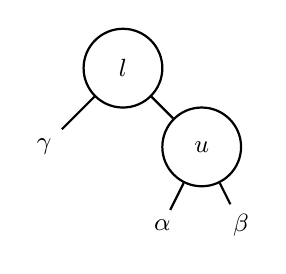
\begin{tikzpicture}[thick,scale=0.5]
        \tikzstyle{every node}=[font=\small]
        \node[every node,circle,draw, minimum size=1cm] (low) at (0, 0) {$l$};
        \node[every node,circle,draw, minimum size=1cm] (up) at (2, -2) {$u$};
        \node (esq) at (-2, -2) {$\gamma$};
        \node[every node] (esqesq) at (1, -4) {$\alpha$};
        \node[every node] (esqdir) at (3, -4) {$\beta$};
        \draw (low) -- (up);
        \draw (esqesq) -- (up);
        \draw (esqdir) -- (up);
        \draw (low) -- (esq);
    \end{tikzpicture}
    \caption[Exemplo de como extrair pontos entre $\low(p)$ e $\up(p)$]{Se $l$ é $\low(p)$ e $u$ é
    $\up(p)$.
    A subárvore $\alpha$ contém todos os pontos que estão entre $\low(p)$ e $\up(p)$ e, portanto,
    corresponde ao conjunto $\Cands(p)$.}
    \label{fig:parestatico:loweup}
\end{figure}